\documentclass[conference]{IEEEtran}
\IEEEoverridecommandlockouts
% The preceding line is only needed to identify funding in the first footnote. If that is unneeded, please comment it out.
\usepackage{cite}
\usepackage{amsmath,amssymb,amsfonts}
\usepackage{algorithmic}
\usepackage{graphicx}
\usepackage{textcomp}
\usepackage{xcolor}
\usepackage{tabularx}
\usepackage{float}
\usepackage{hyperref}
\def\BibTeX{{\rm B\kern-.05em{\sc i\kern-.025em b}\kern-.08em
    T\kern-.1667em\lower.7ex\hbox{E}\kern-.125emX}}
\begin{document}

\title{Large Language Models in Reinforcement Learning - A Comparison of Methods}
\thispagestyle{plain}
\pagestyle{plain}

\author{\IEEEauthorblockN{Adrian Duric}
\IEEEauthorblockA{\textit{Master Student, Dept. of Informatics} \\
\textit{The Faculty of Mathematics}\\
\textit{and Natural Sciences}\\
Oslo, Norway \\
adriandu@ifi.uio.no}
\and
\IEEEauthorblockN{Gregor Kajda}
\IEEEauthorblockA{\textit{Master Student, Dept. of Informatics} \\
\textit{The Faculty of Mathematics}\\
\textit{and Natural Sciences}\\
Oslo, Norway \\
grzegork@ifi.uio.no}
\and
\IEEEauthorblockN{Jonatan Hoffmann Hanssen}
\IEEEauthorblockA{\textit{Master Student, Dept. of Informatics} \\
\textit{The Faculty of Mathematics}\\
\textit{and Natural Sciences}\\
Oslo, Norway \\
jonatahh@ifi.uio.no}
}

\maketitle

\begin{abstract}

Reinforcement Learning (RL) algorithms suffer when rewards are sparse and the state-action space is large. Even tasks which seem relatively simple can prove intractable if the completion of the task requires subtasks to be completed first, or if the reward only comes when the entire task has been completed. In such cases, random exploration is unlikely to lead the agent to discover a solution to the problem. The apparent simplicity of such problems is often due to human intuition, which allow us to quickly see possible solutions to a diverse set of problems. Large Language Models (LLMs) are trained on large corpora of human written text, and have been shown to capture parts of this intuition in many tasks. In recent years, LLMs have been successfully used to aid RL agents in more efficient exploration, and have allowed them to solve problems which previous methods have been unable to. We compare different methods for integrating an LLM into the Deep Learning RL algorithm Proximal Policy Optimization (PPO), and compare their efficiency against each other. 

\end{abstract}

\begin{IEEEkeywords}
large language models, reinforcement learning, minigrid, proximal policy optimization 
\end{IEEEkeywords}

\section{Introduction}

One of the central challenges of reinforcement learning is that rewards are often both extremely rare and delayed, which means that optimizing a reinforcement learning algorithm requires significant trial and error \cite[423]{brunton}. Furthermore, in many problems the state-action spaces are enormous, meaning that uniform exploration is unlikely to find good solutions in a reasonable amount of time. Many methods have been developed to deal with this issue, for example by introducing auxilliary reward functions that use domain knowledge to reward actions which are considered good, or which reward the agent for learning novel skills. However, hand picking which actions to reward can lead to imitation rather than optimal behaviour, and novelty is not always useful \cite[1]{ellm}. In recent years, LLMs have shown remarkable capabilities in problem solving and planning \cite{sparks}, qualities which traditional RL agents often lack. Thus, a new area of research has emerged, which attempts to use the vast amount of human knowledge encoded in these models to improve the performance of reinforcement learning algorithms \cite{survey}. These LLM assisted RL agents have been able to outperform state-of-the-art RL methods in many problems \cite{omni, ellm, idm}.

These papers explore different methods of integrating LLMs into a standard reinforcement learning training loop, from altering the policy directly to introducing an auxilliary reward function. In this paper, we compare both methods in the same environment using the same deep reinforcement algorithm (PPO), and compare their results to each other to explore how LLMs best can be integrated into RL.

\section{Background and Related Work}
\label{background}

RL informed by natural language is a relatively new field, where research before 2018 have been limited to relatively small corpora or synthetic language \cite[1]{survey}. With the introduction of Large Language Models, many new possibilities have opened up, and in recent years there have been many successful integrations of these models into traditional RL \cite{omni, ellm, idm}.


\subsection{Large Language Models as Policy in Reinforcement Learning} 

Among the methods proposed to integrate the LLM, many include ways of making the LLM influence the policy of the RL agent. \cite{omni} considers open-ended learning algorithms in which the value of the agent attempting certain tasks can be evaluated by estimating the the interestingness of the task. The notion of interestingness is then thought of as what task would intuitively be interesting for a human to try in the context of learning in an environment. Some main factors contributing to this interestingness are how likely one is to succeed in doing the task, as well as whether learning the given task may increase the likelihood of succeeding in other tasks. Considering that LLMs are trained on extremely large amounts of human-written text containing human knowledge and intuition, this leads to the idea that if the LLM was told to propose interesting actions for the RL agent to learn in its environment, it could be able to communicate human intuition directly to the agent. This would in turn let the agent learn with increased sample efficiency as the human intuition-based input it receives would make it decide to perform intuitively smarter actions, particularly in the early stages of exploring its environment.

The algorithm proposed in this paper involves prompting the LLM with the agent's state observation, a list of tasks the agent already does well, and a list of available tasks for the LLM to deem as either interesting or boring. After sorting available tasks into interesting and boring ones, it assigns sampling weights to them, giving much higher weights to interesting tasks than boring ones, thus directly influencing the agent's policy by altering probabilities of which action it then chooses to do. In \cite{idm}, another paper proposing using the LLM as a policy influencer, has a similar approach in which the state observation is tokenized and passed to the LLM, though in their experiment, goals and action histories are also tokenized and passed. Here, too, the LLM response is fed back into a task-specific RL model, which in turn influences policy probabilities of certain actions being taken. In general, many of the novel methods suggested involve the LLM suggesting actions for the agent to perform in a given context, and its output influencing the agent policy. 

\subsection{Large Language Models as Reward in Reinforcement Learning}

Another proposed method of involving LLMs in RL, is to have it influence the reward the agent receives for taking certain actions in certain states. In particular, \cite{ellm} cites the infrequency of rewards as a common bottleneck in RL algorithms, due to how long exploratory trajectories often have to be before the agent reaches some desirable state. This holds true especially for large, complex environments, where the probability of reaching favorable states among a huge number of non-favorable states becomes even smaller. Similarly to the papers proposing LLMs to influence policy, this paper too seeks to make use of human intuition and knowledge present in the vast training data that state-of-the-art LLMs have been trained upon, to make the agent prioritize exploring plausibly useful behaviors first, based on some intelligent forethought provided by the LLM.

However, rather than doing so through directly influencing action probabilities in the policy, the paper suggests rewarding the agent if it takes actions that are semantically similar to actions suggested by an LLM. For example, the LLM might recommend the agent to "cut down a tree". If the agent performs the "chop" action at a tree, this action can be described as "chop tree". Using a language model, we can create encodings of these sentences and compare their similarity mathematically. At certain timesteps, the LLM is prompted with a state observation from the agent, and is asked to suggest actions for the agent to take. If the agent then takes actions which are semantically similar to the suggested actions, it receives a reward. Thus, the proposed algorithm makes use of LLMs in two ways: first to generate what the LLM perceives as desirable actions, then later to assess similarity between a natural-language description of the agents action and the previously suggested actions. The first use case in particular utilizes the presence of human intuition in LLMs, as a human would often be able to intuitively figure out what is desirable to achieve in some environment.

\section{Methods}

\subsection{Problem Formulation}

We train a PPO model in a Partially Observable Markov Decision Process (POMDP). A POMDP is defined by a tuple $(S, A, T, R, O, \Omega, \gamma)$. Here, $s \in S$ denotes the state the environment is in and $a \in A$ denotes an action the agent can take. Based on the state and the action taken, the agent receives an observation $o \in \Omega$ which depends on the new environment state and the action taken by $O(o | s, a)$. $T(s' | s, a)$ denotes the state transfer function, which gives a new state based on the previous state and action. $r \in R$ is the reward given by the environment given an action and a state, while $\gamma$ is the discount factor.  The environment we use is part of Minigrid \cite{minigrid}. 

\subsection{Approach}

To evaluate the effectiveness of the integration of LLMs into Reinforcement Learning algorithms, we use the MiniGrid library. Here, we handpick specific environments with varying levels of complexity, to evaluate the effectiveness of our proposed techniques against a standard Actor-Critic PPO, and against each other. % The environments selected are all based in a small sized grid-world, where the agent is surrounded by walls, and has to perform at least one task to complete the game. How difficult an environment is to beat depends on factors such as the shape of the walls, whether the agent has to solve subtasks to finish the game, and the types of subtasks encountered. Moreover, what makes these environments especially well suited for testing our approach is that they are sparse in the context of MiniGrid and BabyAI. This means that the agent will only receive a reward when it finishes the game. It is a well known fact that even state-of-art RL algorithms struggle in very complex and sparse environments. Therefore, it becomes the perfect arena to see if the high generalization capabilites of pre-trained Large Language Models will lead to better results than using only RL methods.


\subsubsection{Standard Proximal Policy Optimization}

Our baseline is the PPO algorithm, which is a policy gradient method that has been established as a state-of-art approach to solving reinforcement learning problems over the last few years. The main idea behind this algorithm is that the new policy is clipped so that it does not move too quickly and too far from the old policy, which helps to avoid changing the policy too drastically during the update. With this simple concept, PPO has outperformed previous methods such as Deep-Q Networks and A2C, while being relatively simple to implement\cite{ppo}.

For the implementation details of our PPO and the hyperparameters used, see the Appendix.


\subsubsection{PPO with LLM Integrated in the Policy Function}

In this case, the LLM is integrated as part of the PPO algorithm, directly influencing the actions taken. This is done as follows: First, the observation is captioned and given as input to the LLM, which is prompted to suggest an action. Then, all actions that the agent could take given the current state are described in natural language. All possible actions are compared with the suggested action, and given a value which denotes their semantic similarity. These values are joined with the logits of the actions, thus influencing the probability weights of each action being taken so that semantically similar actions are weighted higher than others. This is a very direct approach to influencing the agent; if an action is favoured by the LLM in a timestep, this will affect the actions immediately by increasing the chance that this action is sampled. Thus, this method functions as a sort of coach, giving immediate and direct suggestions throughout the episodes. Throughout the paper, we will refer to this as LLM policy influencing.

\subsubsection{PPO with LLM Integrated in the Reward Function}

The agent is trained as in the baseline. The agent's state observation is encoded to natural text, and sent as part of a prompt to the LLM at every timestep. In addition to the state observation, the LLM is also asked to respond with a list of recommended actions for the agent to perform. The agent then acts independently of the LLM for that timestep, as dictated by the baseline RL algorithm it is trained with. As it does so, its chosen action is encoded to natural text. Then, the LLM is used as a tool for semantic similarity comparison, comparing its own formerly proposed action to the action performed by the agent. Finally, high semantic similarity gives an additional pseudo-reward which is added to the reward of the environment. Compared to the policy influencing method above, this approach is less direct, as the policy is only indirectly affected by the LLM through these additional rewards, which only take effect when the policy is updated through backpropogation after an entire episode is completed. Thus, this method functions more as an advisor, influencing the policy in a more long term capacity than the coaching of the policy influencer. Throughout the paper, we will refer to this as LLM reward shaping.

\subsubsection{PPO with both LLM reward shaping and LLM policy influencing}

Finally, we combine the two LLM integrations, hoping to combine the direct influence of our policy integration with the more indirect reward shaping. Thus, we are affecting the policy in two ways: Through reward shaping, we are causing the policy to update to better attain the aforementioned pseudo-rewards, which will encourage completing of subgoals which are necessary to complete the actual goal of the environment, but which do not give out intermediate rewards. Through policy influencing, we are nudging the agent to take favorable actions by directly altering the action probabilities, which will make it more likely that the agent completes the given task and receives an actual reward from the environment. Thus, the agent will more quickly discover the correct policy. We call this the \textbf{Actor-Advisor-Critic-Coach} method, or \textbf{A2C2} for short.


\subsection{Language Models}

In both these cases, we need two language models; one to generate the suggestions and one to generate semantic similarity values.

For text generation, we have decided utilize an LLM from the Llama open-source family of language models developed by Meta AI, first released in Febraury, 2023. Specifically, we chose Llama 2, which has been trained using 40\% more data than its predecessor Llama 1, and has double the context length\cite{llama}. In the experiments presented below, we use the smallest version of Llama2, with 7 billion parameters, which we download to run locally and reduce the bottleneck effect of having to call an API to a model hosted by someone else. The reason for not using any of the larger Llama 2 models is simply the hardware limitation we face, with the 7B model requiring 19GB of VRAM to be run. 

Some research papers propose fine-tuning of LLMs as means of leveraging the capabilites of the language models for decision-making purposes even further \cite{grounding}. Our plan of action, on the other hand, aims at evaluating the efficacy of the LLM without any previous pre-tuning. From the perspective of reinforcement learning, this is the appropriate course of action, as the LLM should not possess any previous knowledge about the task at hand, just like the agent should not. In addtion, the act of fine-tuning LLM is a rather time-comsuming process, requiring the generation and structuring of a new dataset, and also vast hardware resources. 

Instead of fine tuning the LLM, we use few-shot learning when prompting, giving the LLM a few examples of observations and correct corresponding action recommendations. This is an effective way to guide the LLM for our specific purposes without requiring us to retrain the entire network.

For generating semantic similarity values, we use Sentence-Bert \cite{bert} for generating encoding vectors, and perform a cosine similarity calculation of the two sentence encodings. This gives a value between $-1$ and $1$, where two sentences with the exact same encoding have a cosine similarity of $1$.


\section{Experiments}

We perform experiments to compare different methods of integrating LLMs with the PPO algorithm, specifically comparing their ability to guide the early exploration of an RL model in a reward-sparse environment. Even state-of-art RL algorithms may struggle in such environments. Therefore, it is the perfect arena to see if the high generalization capabilites of pre-trained Large Language Models will lead to better results over using only RL methods.

\subsection{Minigrid Environments}

For our experiments, we choose the Minigrid library. The Minigrid library contains simple grid world environments. An important characteristic of all these environments is that they only give reward on the completion of the goal of the environment. In other words, the environment only ever gives out a single reward per episode, given that the agent completes its task. Goals in Minigrid are often simple tasks, such as "unlock the door", "go to the goal", "pick up the red chest", etc. Completing these goals often requires the completion of subtasks; going to the goal might require opening a door, and opening the door might require picking up a key. These environments are partially observable, which means that the agent only receives a seven by seven observation grid, not the entire grid. Figure \ref{doorkeyenv}, shows a typical minigrid environment. In this case, the agent (the red arrow) only sees the left room, and does not know where the goal is.

\begin{figure}[h]
\centerline{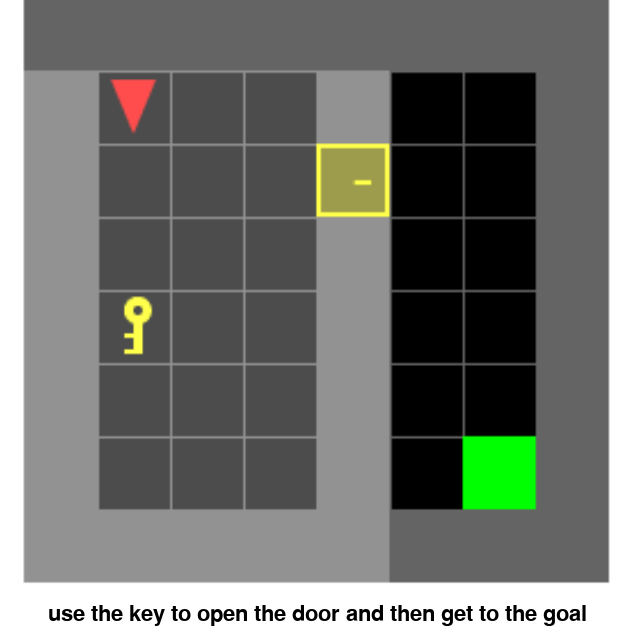
\includegraphics[width=3.25in]{figure/doorkeyenv.png}}
\caption{The Minigrid DoorKey environment}
\label{doorkeyenv}
\end{figure}

A more complicated environment can be seen in figure \ref{blockedunlockpickupenv}. Completing the goal requires picking up the ball and dropping it somewhere else, picking up the key, using it to unlock the door, dropping the key (the agent can only carry one item at once) and finally picking up the box. With no intermediate rewards, this is a very difficult task for traditional RL methods. The exact configuration of Minigrid environments is random; the position of the agent, the placement of the walls and items within the grid all vary from episode to episode.

\begin{figure}[h]
\centerline{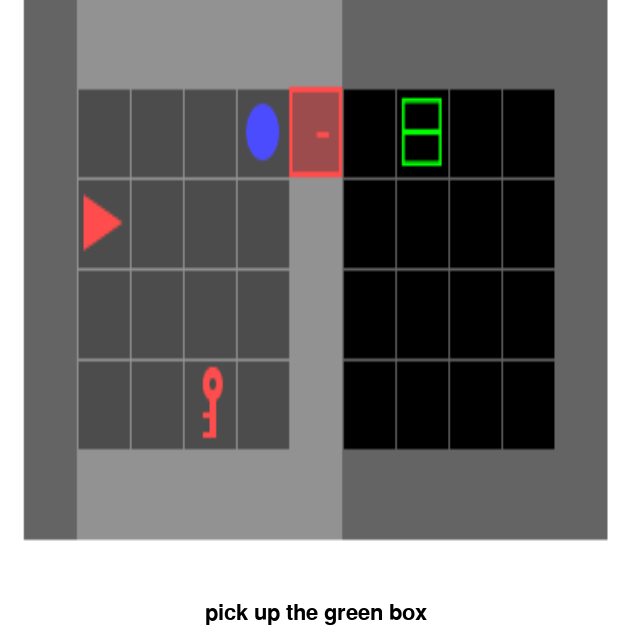
\includegraphics[width=3.25in]{figure/blockedunlockpickupenv.png}}
\caption{The Minigrid BlockedUnlockPickup environment}
\label{blockedunlockpickupenv}
\end{figure}

Some environments can only be effectively solved by relying on language (for example, environments where the goal text describes a specific object to be picked up, which changes every time), while others can be solved without (for example, if the goal always is to pick up a key). We only use environments that can be solved without language, so that the baseline PPO algorithm is not at an unfair disadvantage.

\subsection{Our chosen environments}

We select three different Minigrid environments with increasing complexity; Empty, DoorKey and UnlockPickup. For each environment we test our four different models; PPO with no LLM integration, PPO with LLM reward shaping and PPO with LLM policy influencing. All methods use the same hyperparameters for the PPO, which can be found in the appendix. For each of these methods, we run PPO for 2000 (200 for Empty) episodes of 1024 steps, and track the reward\footnote{The true environment reward, not including pseudo-rewards given by the LLM in reward shaping} received for each one. We do this eight times per method, and compare the average results per episode against each other.

\subsubsection{Empty environment}

This environment is the simplest possible, consisting of an empty room with a single goal in the bottom right corner. This environment contains no stochasticity; the agent and goal always start in the same positions. Despite its simplicity, there is still potential for LLM integration to improve the early phases of training, because the room is 15 by 15 tiles, which means that receiving any reward requires a significant amount of exploration. The environment is seen in figure \ref{emptyenv}.

\begin{figure}[h]
\centerline{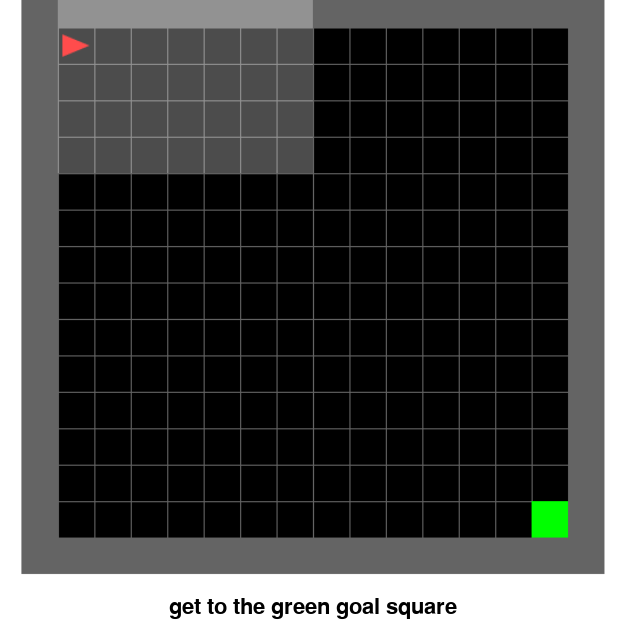
\includegraphics[width=3.25in]{figure/emptyenv.png}}
\caption{The Minigrid Empty Environment}
\label{emptyenv}
\end{figure}

\subsubsection{DoorKey environment}

This environment consists of two rooms separated by a locked door. Fig \ref{doorkeyenv} shows an example configuration. The agent starts in one room, while the goal square is in the other. The agent must pick up a key in the starting room, and use it on the door to gain access to the room containing the goal. This environment thus contains two subgoals; picking up the key and using it to unlock the door.

\subsubsection{UnlockPickup environment}

This environment is quite similar to the DoorKey environment. Fig \ref{unlockpickupenv} shows an example configuration. The difference is that after unlocking the door, the agent must now pick up a chest instead of walking to a goal square. Because the agent can only hold one item at a time, this requires dropping the key on an empty square, which introduces another subtask. Chests can also be opened like doors, but this removes the chest from the game and thus causes and instant failure of the task, as it can no longer be picked up. Thus, the agent must learn that using a key on a door is a valuable subtask, while using it on a chest is a bad idea. This added complexity makes it a much more difficult task than the previous two.

\section{Results}

\subsection{Empty Environment}

In this simple environment, we see that both LLM reward shaping, LLM policy influencing and A2C2 outperform the baseline model. Averaging over all episodes for all eight runs, we find that reward shaping increases the mean reward received by $10\%$ over the baseline, with a lower standard deviation in rewards received per run of $0.12$. Policy influencing scores even higher at $32\%$ over the baseline, with an even lower standard deviation of $0.09$. Finally, A2C2 performs the best of the four with a $37\%$ increase in average reward over the baseline model, and the lowest standard deviation of $0.04$

Notably, both policy influencing and A2C2 receive much higher rewards than reward shaping and the baseline right from the first episode. This makes sense as the environment is so simple that the LLM seems not to have any problem giving sensible instructions to directly influence the policy most of the time. However, we notice from the graph that policy influencing alone consistently gives a significant dip in received reward after the first few episodes, which it later compensates for, following a similar trajectory to that of reward shaping after about 50 episodes. We believe this could be a sign of the policy influencing being somewhat overly influential in changing the logits early on, because the logits initially have low values. As the PPO learns the environment, the magnitude of the logits increases, which at some point leads to conflicting contributions to the logits from the LLM and from the PPO. As the dip stops and performance increases again, this is likely due to the PPO becoming more influencing than the LLM after having started to learn the environment properly. We also notice that this dip is completely removed with A2C2, which could signify that the added reward shaping helps the PPO learn faster, enabling it to increase the influence from PPO on the logits faster.

\begin{figure}[h]
\centerline{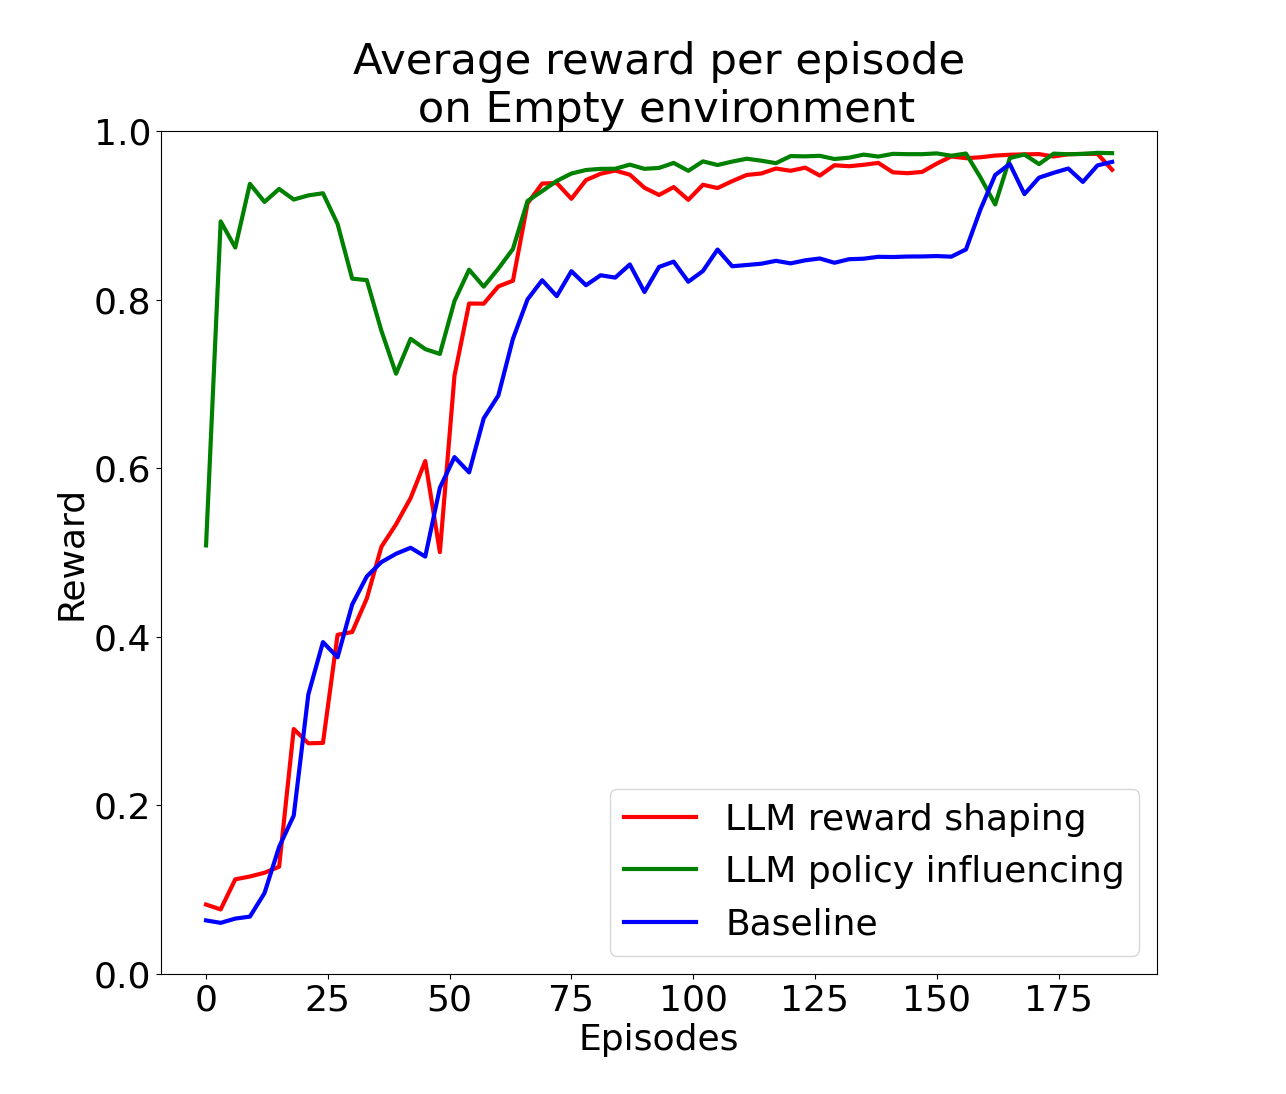
\includegraphics[width=3.25in]{figure/emptyresults.png}}
\caption{Reward per episode for the four different methods in the Empty environment}
\label{doorkeyresults}
\end{figure}

\begin{table}[h]
\caption{All results on Empty environment}
\begin{center}
\label{emptytable}
\begin{tabular}{c | c c c}
Method & Mean reward & Std reward & Increase over baseline \\
\hline
Reward shaping & 0.76 & 0.12 & 10\% \\
Policy influencing & 0.91 & 0.09 & 32\% \\
Both & 0.95 & 0.04 & 37\% \\
Baseline & 0.69 & 0.28 & 0\% \\
\end{tabular}
\end{center}
\end{table}


\subsection{DoorKey environment}

As we can see from Figure \ref{doorkeyresults}, we see impressive results from our LLM integration in this environment as well, especially from reward shaping and A2C2. For the mean and standard deviation of all methods, see table \ref{doorkeytable}.

\begin{table}[h]
\caption{All results on DoorKey environment}
\begin{center}
\label{doorkeytable}
\begin{tabular}{c | c c c}
Method & Mean reward & Std reward & Increase over baseline \\
\hline
Baseline & 0.99 & 1 & 0\% \\
Reward shaping & 0.99 & 1 & 30\% \\
Policy influencing & 0.99 & 1 & -7\% \\
Both & 0.99 & 1 & 36\% \\
\end{tabular}
\end{center}
\end{table}

LLM reward shaping gives a noticable improvement to the performance of the model, not just in the early stages of training, but throughout the entire training process. Averaging over all episodes of all eight runs per model, we find that LLM reward shaping receives $24\%$ more reward per episode than PPO trained without LLM rewards. Furthermore, this is an improvement that comes at very little computational cost, because LLM responses can be cached between runs. Of the eight runs on this environment using LLM reward shaping, the last three runs never queried the LLM at all, only relying on the cache of previous answers.

Looking at LLM policy influencing, we see that it has resulted in somewhat worse results than using the PPO baseline. Averaging per episode over all eight runs shows that LLM policy influencing only achieves $89\%$ of the reward amount per episode that the baseline achieves. Judging from the graph, it may seem that policy influencing may have given some initial learning advantage, but ultimately slows learning for the agent further on. The method also gives the highest standard deviation of reward given per episode of the three compared so far, at $0.25$. As with reward shaping, we have also used caching of LLM responses to significantly decrease the computational overhead cost to a minimum. 

However, the results from both of these methods are eclipsed by the results from combining LLM reward shaping and policy influencing together in our A2C2 model. Averaging over 8 runs, we observe a $34\%$ increase in reward from the environment compared to PPO alone, $8\%$ higher than reward shaping and $43\%$ higher than policy influencing, with the lowest standard deviation of all methods, at $0.22$. Clearly, the combination of immediate direct suggestions from the policy influencer and long term indirect suggestions from the reward shaper is a favourable way of integrating the LLM with PPO, which gives results which are better than the sum of its parts, not only in the simple Empty environment, but also in more complicated environments like DoorKey.

\begin{figure}[h]
\centerline{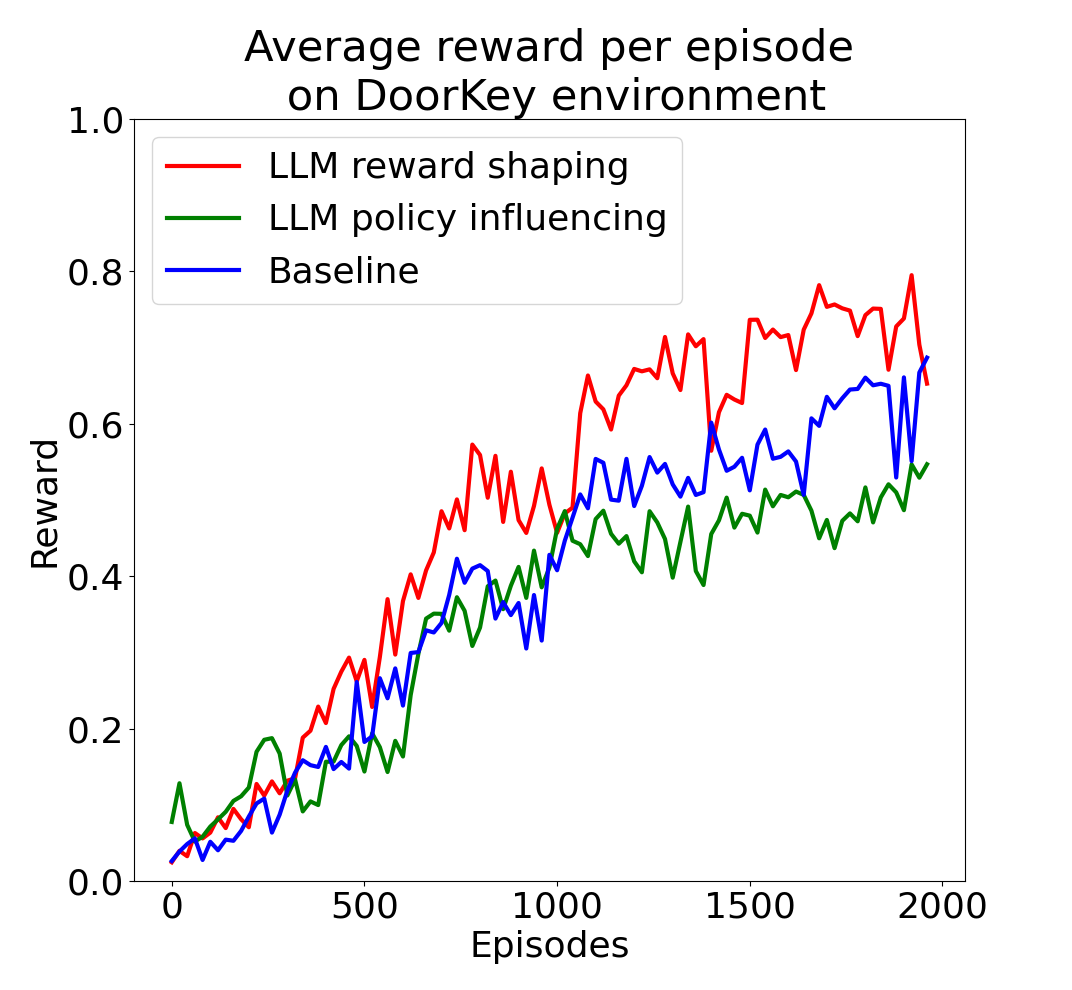
\includegraphics[width=3.25in]{figure/doorkeyresults.png}}
\caption{Reward per episode for the four different methods in the DoorKey environment}
\label{doorkeyresults}
\end{figure}

\subsection{Unlock Pickup environment}

The Unlock Pickup environment is an even more complex environment than DoorKey, requiring a much longer string of actions to give out a reward. As may be anticipated, this added complexity makes the average reward much lower, and we see that all methods struggle (figure \ref{unlockpickupresults}).

\begin{figure}[h]
\centerline{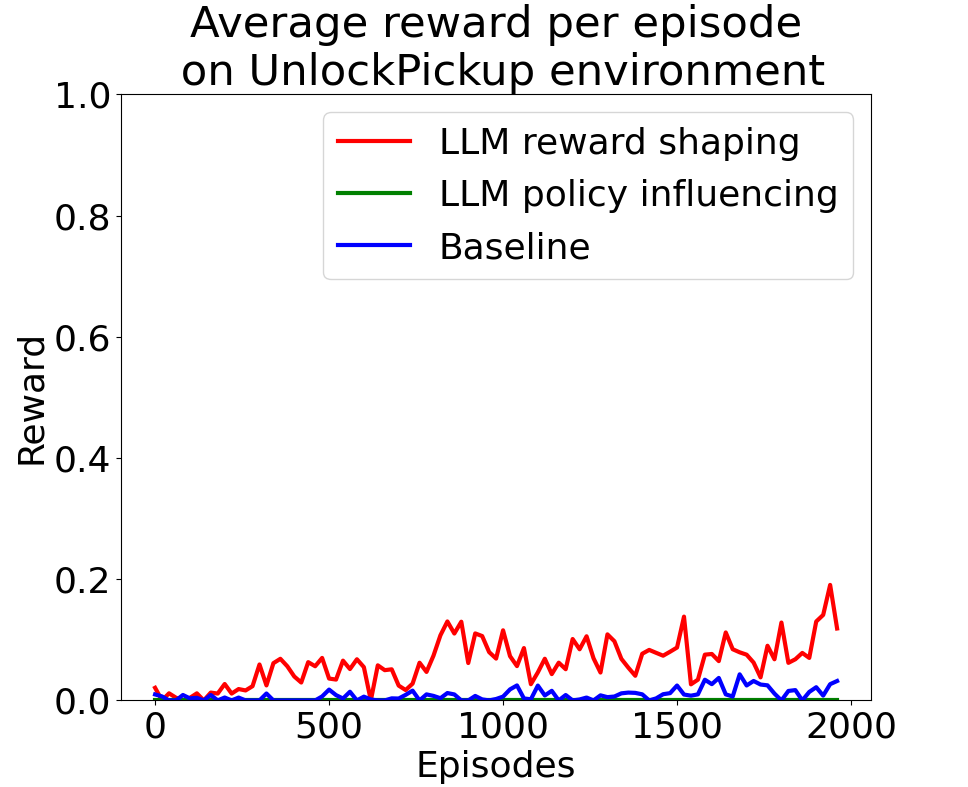
\includegraphics[width=3.25in]{figure/unlockpickupresults.png}}
\caption{Reward per episode for the four different methods in the UnlockPickup environment}
\label{unlockpickupresults}
\end{figure}

As we can see, LLM performs the best overall, and performs much better than vanilla PPO, which struggles to learn the correct policy in this complex environment. Given the terrible performance of the baseline, LLM reward shaping achieved a percentage increase of over $700\%$, which is not that impressive when the average reward from the baseline was close to zero. The baseline achieved an average reward of $0.0089$ (with a standard deviation of $0.015$), while LLM reward shaping achieved an average reward of $0.062$ (with a standard deviation of $0.081$). See table \ref{unlockpickuptable}.

\begin{table}[h]
\caption{All results on UnlockPickup environment}
\begin{center}
\label{unlockpickuptable}
\begin{tabular}{c | c c c}
Method & Mean reward & Std reward & Increase over baseline \\
\hline
Baseline & 0.99 & 1 & 0\% \\
Reward shaping & 0.99 & 1 & 30\% \\
Policy influencing & 0.99 & 1 & -7\% \\
Both & 0.99 & 1 & 36\% \\
\end{tabular}
\end{center}
\end{table}

As we can see, policy influencing struggles in this environment as well, performing even worse than the baseline. Policy influencing received a mean average score of NUMBER, which is PERCENT lower than the baseline. In this complicated environment, it may that suboptimal responses from the LLM have high chance to ruin the agent's chance to complete the goal, for example by suggesting to open the box instead of picking it up. As explained earlier, this instantly loses the game by removing the box from the game.

Our A2C2 performs much better than just policy influencing, but we are not here able to combine the two LLM integrations to receive a performance higher than the sum of its parts. Here we receive a score of NUMBER, which is higher than the baseline and policy influencing, but not higher than reward shaping by itself. It may be that in this case, the performance of policy influencing is so poor that the combination is not able to utilize the best of both methods, instead only being dragged down by poor suggestions.

\subsection{Inspecting the LLM responses}

Having looked at the performance of our different models, we can see that the suggestions from the LLM have positive effects in many cases, while also sometimes being detrimental. We now inspect some sample responses from the LLM, to gain deeper understanding of how the LLM is effecting the agent.

\subsubsection{Empty}

From table \ref{emptyresponses} we see that the suggestions are very good, which explain the great performance all LLM integrations show.

\begin{table}[h]
\caption{All results on UnlockPickup environment}
\begin{center}
\label{unlockpickuptable}
\begin{tabular}{c | c}
Prompt & Response \\
\hline
My goal is: get to the green goal square. I see a green goal LEFT and FORWARD." & "move forward."
\end{tabular}
\end{center}
\end{table}


\section{Discussion, Future Work and Conclusion}

As shown in the previously referenced work (\ref{background}), the integration of a Large Language Model into the Reinforcement Learning framework can improve network performance. There are various ways to do this, and our work attempts to compare two main methodologies of integrating the LLM, namely through reward shaping and policy influencing. We have implemented algorithms to perform this on top of a PPO baseline, as well as a combination of the two, and have measured varying results across environments of different complexities.

Our reward shaping algorithm did best in the more complex environments (DoorKey and Unlock Pickup), while policy influencing performed better in the simpler Empty environment. A possible explanation for this could lie in the details of how the algorithms impact choice of action. LLM reward shaping does not directly impact decision making at all; it only impacts the reward function, meaning the mechanism that dictates which action is taken is still solely the actor network present in PPO. This means that reward shaping does not introduce any risk of the agent choosing a suboptimal action directly due to being told to do so by the LLM. Learning which action to take is still done through the same process of trial and error as in classical RL.

However, the causality behind which action is taken is different in LLM policy influencing; the LLM suggestions are added directly to the logits used to calculate probabilities of each action, meaning that the LLM directly influences the decision making process. Every time the LLM suggests performing a suboptimal action, this impacts the sampled action, regardless whether the PPO baseline has learned that another action is better or not. Over time, this may lead to the PPO not being able to explore other actions than the ones proposed by the LLM, thus making the PPO learn slower than if it was allowed to choose actions on its own. In other words, the LLM may have too much impact in the decision making when performing policy influencing, making the algorithm prone to errors from the LLM.

A natural suggestion for how to improve the performance of LLM policy influencing in the future thus becomes to decrease the influence from the LLM over time, letting the PPO choose on its own as learning progresses. One way of doing this is through annealing of the LLM values added to the logits. This can be combined with experimenting with a hyperparameter determining how the LLM values should be weighted at the beginning of training. We have attempted to do this, but have encountered programmatic issues regarding scaling; the logits change in magnitude over time, and a fitting way of dynamically changing the LLM contributions to the logits has to be found.We believe this is what causes the noticable dip in performance that happens after some initial rollouts in the policy influencing results.

Overall, we found that the LLM can be a valuable asset in the RL framework, but that a balance must be struck regarding how significantly it should influence the learning process.

\section*{Ethics Statement}

In accordance with the NeurIPS Code of Ethics \cite{ethics}, we outline ethical considerations related to this project, covering potential consequences from the research, and how potential risks may be mitigated. Considering that our research does not involve participants nor sensitive data, concerns related to how such factors are treated will not be discussed.

\subsection{Societal Impact and Potential Harmful Consequences}

Due to how this research project revolves around the integration of LLMs in the RL domain, many of the same concerns that exist in the domain of LLMs themselves are extended to the RL domain. A major concern is that of safety; if the RL agent is to act in an environment where failure to act optimally could be critical, it is paramount that the agent does not enter bad states due to the existing randomness in the RL framework. The LLM in itself predicts stochastically, and thus may add even more noise to the framework. In the worst case, it could amplify probabilities of the agent choosing dangerous actions due to this added noise.

Another topic of concern is that of bias and fairness; the premise for why an LLM might help an RL agent in a large environment is because of its inherent human knowledge, stemming from the human-written texts it has been trained upon. However, human-written texts are an obvious potential source to biased opinions, and the LLM may have learned such biased and/or unfair opinions. Then, in an example where the RL agent is deployed in environments where an ethical choice has to be made, this choice could be influenced by whatever bias may be present in what the LLM suggests to the agent.

\subsection{Impact Mitigation Measures}

As is exemplified above, major ethical concerns regarding the use of our proposed algorithms arise when they are deployed for critical tasks, for instance tasks in real-life dangerous environments, or environments where ethical considerations have to be addressed. Therefore, an agent trained on our proposed RL framework for such critical tasks should be carefully tested before deployment to see if, and how often, critical deviations occur.

In the further development of this and similar algorithms, we also consider it essential to put effort into trying to understand the causality behind certain actions being taken, as is being done in the field of explainable artificial intelligence (XAI). When involving a major ML framework like that of LLMs into RL, we would ideally want to see exactly where and how much the LLM contributes to the RL networks being updated. This would, in turn, help in the work to mitigate whatever biases and variance that may be added to the RL framework from integrating the LLM.

\section*{Acknowledgment}

We would like to acknowledge the ROBIN research group at the University of Oslo Dept. of Informatics, who have arranged for us to be able to undertake this research and gain valuable experience. In particular, we would like to thank our supervisors Katrine Nergård and Kai Olav Ellefsen for their help and guidance in this project.

\bibliographystyle{apalike}
\bibliography{bibliography}


\section*{Appendix}

\begin{figure}[h]
\centerline{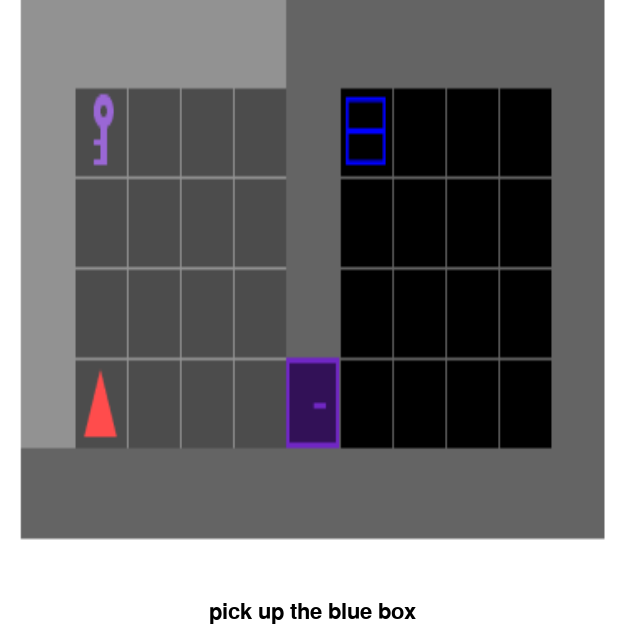
\includegraphics[width=3.25in]{figure/unlockpickupenv.png}}
\caption{The Minigrid UnlockPickup environment}
\label{unlockpickupenv}
\end{figure}

\begin{table}[h]
\caption{PPO hyperparameters}
\begin{center}
\label{hyperparams_transposed}
\begin{tabular}{c | c}
Parameter & Value \\
\hline
Gamma & 0.99 \\
Steps/episode & 1024 \\
Epochs/episode & 10 \\
Batches/epoch & 8 \\
Clip & 0.2 \\
Value loss coeff. & 0.3 \\
Entropy coeff. & 0 \\
Learning rate & 3.0e-4 \\
\end{tabular}
\end{center}
\end{table}



\end{document}
